\documentclass[10pt,pdf,hyperref={unicode}]{beamer}

% \documentclass[aspectratio=43]{beamer}
% \documentclass[aspectratio=1610]{beamer}
% \documentclass[aspectratio=169]{beamer}

\usepackage[english,russian]{babel}
%\usepackage[intlimits]{amsmath}
\usepackage{lmodern}
\usepackage[labelsep=period]{caption}
% подключаем кириллицу 
\usepackage[T2A]{fontenc}
\usepackage[utf8]{inputenc}

\usepackage{graphicx}
\graphicspath{{pictures/}}
\DeclareGraphicsExtensions{.pdf,.png,.jpg}



% отключить клавиши навигации
\setbeamertemplate{navigation symbols}{}

% тема оформления
\usetheme{Berlin}
% цветовая схема
 \usecolortheme{default}

\title{Геометрическая оптика}   
%\subtitle{устройство и применение}
\author{Фазлиахметова Олеся Камилевна} 
\date{\today} 


\begin{document}

	\begin{frame}
\titlepage
	\end{frame} 



	\begin{frame}
\frametitle{Содержание и основные вопросы} 
\tableofcontents
	\end{frame}



	\begin{frame}
\section{Применимость}
\frametitle{Применимость геометрической оптики} 

%Явления интерференции и дифракции света показывают, что распространение света представляет собой волновой процесс. С помощью волновой теории можно решать задачи о распространении света как в однородной среде, так и через любую оптическую систему. Однако в очень многих областях, имеющих важное практическое значение, например, в теории формировании светового пучка и образования изображения, решение
%можно получить гораздо более простым путём с помощью представлений
%геометрической оптики.
%Геометрическая оптика оперирует понятием отдельных световых лучей,
%подчиняющихся известным законам преломления и отражения, и
%независимых друг от друга.
%При попытке на практике получить тонкий световой луч при помощи
%диафрагмы или последовательности диафрагм неизбежно реализуется
%дифракционное расширение светового пучка. Угол расширения можно
%приближенно оценить следующим образом: φ=λ/D, где λ – длина волны света,
%D – диаметр отверстия в диафрагме. Таким образом, тонкий нерасходящийся
%световой пучок («луч») можно получить только в том случае, когда λ/D→0.
%Именно в этом приближении верны утверждения, получаемые в рамках
%геометрической оптики.
%В рамках данной лабораторной работы соотношение λ/D<<1
%выполняется, поскольку геометрические размеры используемых оптических
%элементов (линз, пластин и т.д.) D существенно превышают длины волн
%светового диапазона, в связи с чем уместно применение формул и
%соотношений, полученных в рамках приближения геометрической оптики.
%Тем не менее, следует помнить, что лабораторная работа сопровождается
%проявлением дифракционных эффектов, например, отсутствием резких
%границ теней, т.е. частичным размытием границы света и тени на экране, где
%происходит фокусировка изображения.
\begin{block}{Угол расширения}
\[\phi=\frac {\lambda}{D}\]
\end{block}
Тонкий нерасходящийся световой пучок («луч») можно получить только в том случае, когда $\frac {\lambda}{D}\rightarrow0.$
	\end{frame}



	\begin{frame}
\frametitle{Цель работы} 
\section{Цели работы}

Перед началом работы были поставлены следующие задачи:

\begin{enumerate}
	
	\item Ознакомиться с базовыми оптическими приборами, а также некоторыми методами установки фокусных расстояний линз и оптических систем. 
	
	\item Определить фокусное расстояние плоской положительной линзы различными способами.
	
	\item Определить фокусное расстояние оптической системы с помощью метода Аббе.
	
	\item Определить фокусное расстояние и положение главных плоскостей системы линз.
	
	\item Определить угловое увеличение телескопа.
\end{enumerate}
\end{frame}



	\begin{frame}
\frametitle{Опыт 1 -- опеределение фокусного расстояния} 
\section{Определение F}
%Если расстояние между линзой и объектом будет в точности равно фокусному расстоянию, то изображение объекта будет располагаться на бесконечности. Если за линзой расположить плоское зеркало, то лучи, прошедшие сквозь линзу, отразятся от зеркала и, вновь пройдя сквозь линзу, сформируют перевернутое изображение объекта без увеличения в фокальной плоскости, т.е. в плоскости, в которой расположен объект. Схема представлена на  Рис. \ref{fig:1_1}.

%Для того, чтобы было проще определить, что изображение оказалось равновеликим, предмет был такой формы, чтобы его перевернутое равновеликое изображение дополняло его до круга.


\begin{figure}[H]
	\centering
	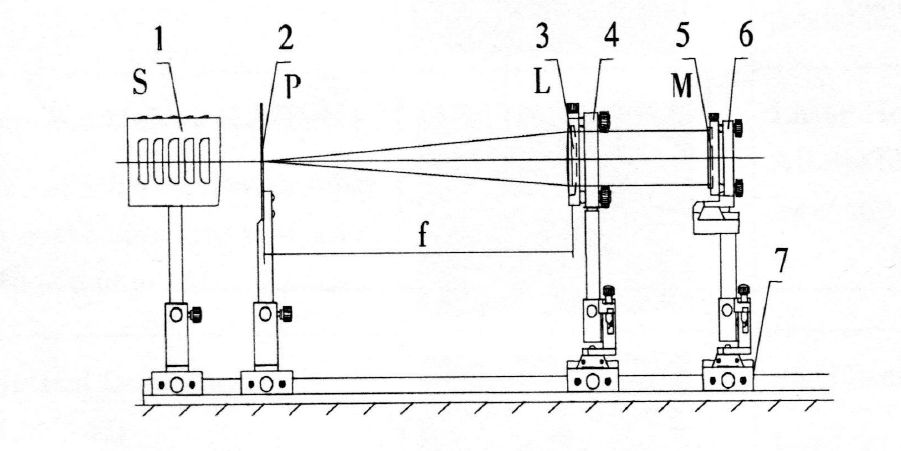
\includegraphics[width=0.7\linewidth]{1}
	\caption{ При помощи зеркала
%Схема расположения оптических элементов в опыте по определению фокусного расстояния линзы с использованием плоского зеркала. На рисунке изображены следующие элементы: 1~-- осветитель S; 2~-- объект P (LMP-141); 3~-- собирающая линза L ($f=150$ мм); 4, 6~-- двухосевой держатель оптических элементов (LMP-07); 5~-- плоское зеркало М 
}
	\label{fig:1_1}
\end{figure}
\end{frame}





	\begin{frame}
\frametitle{Данные опыта 1} 
%Ход работы заключался в следующем: мы собрали установку (см.  Рис. \ref{fig:1_1}) , провели юстировку. Двигали линзу L вдоль оптической скамьи, пока не получили четкое (и равное по размеру с объектом) перевернутое изображение объекта на пластине P. Провели измерение.

%Для верности линза была перевернута другой стороной и поставлена в необходимое положение еще раз.

\begin{center}
	\begin{tabular}[H]{|c|c|}
		\hline
		№ измерения & F, мм \\
		\hline
		1 & $145 \pm 0.5$ \\
		\hline
		2 & $148 \pm 0.5$ \\
		\hline
		3 & $150 \pm 0.5$ \\
		\hline
		4 & $145 \pm 0.5$ \\
		\hline
		5 & $150 \pm 0.5$ \\
		\hline
		6 & $150 \pm 0.5$ \\
		\hline
	\end{tabular}
\end{center}
Таким образом, усреднив полученные значения, получаем:
\begin{equation*}
	F = 148 \pm 2 \text{ мм}
\end{equation*}
\end{frame}





	\begin{frame}
\frametitle{Определение фокусного расстояния с помощью экрана}
%Этот способ основывается на том, что в случае, когда расстояние от предмета до экрана превышает $4F$, появляется два положения линзы, в которых получается четкое изображение предмета на экране. (в одном случае уменьшенное, в другом -- увеличенное). Из соображений симметрии ясно, что $a_1=a_2'$ и $a_2=a_1'$. Схема опыта представлена на Рис. \ref{fig:1_2}
%Пусть $а$ --- расстояние от предмета до линзы, $f$ --- расстояние от линзы до изображения, $L$ --- расстояние между линзой и изображением (экраном).  Пусть расстояние между положениями изображения $l$. Тогда:

\begin{align*}
	a_1 &= \frac{L - l}{2} \\
	a_2 &= \frac{L + l}{2}
\end{align*}

%С учетом формулы тонкой линзы, получим:

\begin{equation}
	F = \frac{L^2 - l^2}{4L}
\end{equation}

\begin{figure}[H]
	\centering
	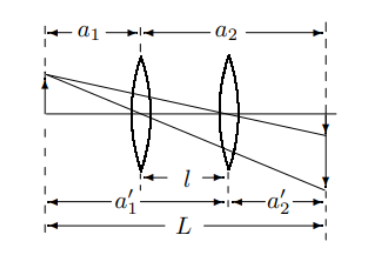
\includegraphics[width=0.4\linewidth]{3}
	\caption{Измерение фокусного расстояния тонкой положительной линзы}
	\label{fig:1_3}
\end{figure}

\end{frame}



	\begin{frame}
\frametitle{Данные}
%Таким образом, необходимо определить необходимую сдвижку линзы $l$ из первого положения, в котором появляется четкое изображение предмета, до второго при заданном $L$. В ходе работы мы перемещали вдоль оптической скамьи линзу, пока не нашли четкое изображение объекта P на экране H. 

%В ходе эксперимента были получены следующие результаты:

\begin{center}
	\begin{tabular}{|c|c|c|c|}
		\hline
		№ серии & $L$, мм & $l$, мм & $F$, мм  \\
		\hline
		1 & $650 \pm 0.5$ & $195 \pm 0.5$ & $148 \pm 0.5$  \\
		\hline
		2 & $700 \pm 0.5$ & $273 \pm 0.5$ & $149 \pm 0.5$ \\
		\hline
		3 & $800 \pm 0.5$ & $399 \pm 0.5$ & $151 \pm 0.5$  \\
		\hline
		\multicolumn{4}{|c|} {Поворот на 180$^\circ$ }\\
		\hline
		1 & $700 \pm 0.5$ & $269 \pm 0.5$ & $149.2 \pm 0.5$  \\
		\hline
		2 & $650 \pm 0.5$ & $195 \pm 0.5$ & $147.9 \pm 0.5$ \\
		\hline
		3 & $850 \pm 0.5$ & $469 \pm 0.5$ & $148 \pm 0.5$  \\
		\hline
	\end{tabular}
\end{center}
%После усреднения всех полученных фокусных расстояний, получаем: % Посчитать погрешность и как следствие число знаков

\begin{equation*}
	F = 148.85 \pm1.21 \text{ мм}
\end{equation*}
\end{frame}


\begin{frame}
\section{Метод Аббе}
\frametitle{Метод Аббе} 
%Фокусное расстояние оптической системы может быть измерено также с помощью метода Аббе. Получим расчетную формулу:

%Предположим, что линейный размер предмета равен $y$, а находится он на расстоянии $x_1$ от главного фокуса $F$ положительной оптической системы. Изображение предмета в таком случае имеет размер $y_1$, а линейное увеличение равно $\beta_1 = y_1 / y = F / x$. Если же теперь передвинуть предмет на небольшое расстояние $\Delta x$, то увеличение изменится и станет равным $\beta_2 = y_2 / y = F / x$. В таком случае, легко получить:

\begin{equation}
	F = \frac{\Delta x}{\frac{1}{\beta_1} - \frac{1}{\beta_2}}
	\label{eq:1}
\end{equation}
%Таким образом, необходимо определить линейное увеличение $\beta_1$ в одном положении линзы, и линейное увеличение $\beta_2$ в сдвинутом относительно первого на $\Delta x$. Схема опыта представлена на Рис. \ref{fig:2}.

\begin{figure}[H]
	\centering
	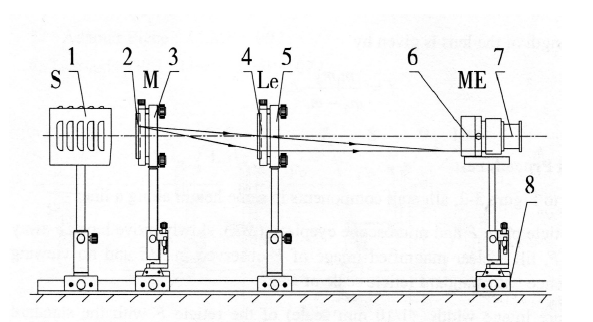
\includegraphics[width=0.7\linewidth]{4}
	\caption{Метод Аббе} %Схема расположения оптических элементов в опыте по определению фокусного расстояния линзы с помощью метода Аббе. На рисунке изображены следующие элементы: 1~-- осветитель S; 2~-- слайд с делениями M (Reticle); 3~-- держатель бипризм (LMP-41); 4~-- линза Le ($f=35$ мм); 5~-- двухосевой держатель оптических элементов (LMP-07); 6~-- окуляр микроскопа МЕ; 7~-- держатель микроскопа (LMP-09)}
	\label{fig:2}
\end{figure}
\end{frame}



\begin{frame}
\frametitle{Метод Аббе} 

%В результате экспериментов были полученные следующие данные:

\begin{center}
	\begin{tabular}{|c|c|c|c|c|}
		\hline
		 № & $\beta_1$ & $\Delta x$, мм & $\beta_2$ & F, мм \\
		\hline
		1 & 1.2 & 10 & $\frac 5 3$ & 42.8 \\
		\hline
		2 & $\frac 4 3$ & 10 & 1 & 40\\
		\hline
		3 & 1.1 & 11 & 1.5 & 33 \\
		\hline
	\end{tabular}
\end{center}

%Тогда, с учетом формулы (\ref{eq:1}), получаем значение фокусного расстояния:

\begin{equation*} % Погрешность
	F = 38.6 \pm 4.1\text{ мм}
\end{equation*}
\end{frame}


\begin{frame}
\section{Оптическая система}
\frametitle{Оптическая система} 

%Рассмотрим оптическую систему, которая состоит из двух центрированных собирающих линз, расположенных на известном расстоянии друг от друга. 

%Если система состоит из двух собирающих линз, то фокусное расстояние системы можно рассчитать следующим образом:

\begin{equation}
	\frac{1}{F} = \frac{1}{F_1} + \frac{1}{F_2} - \frac{l_{12}}{F_1 F_2}
	\label{eq:2}
\end{equation}

%Здесь $l_{12} = 40 \pm 0.5$ мм --- расстояние между линзами.


\begin{figure}[H]
	\centering
	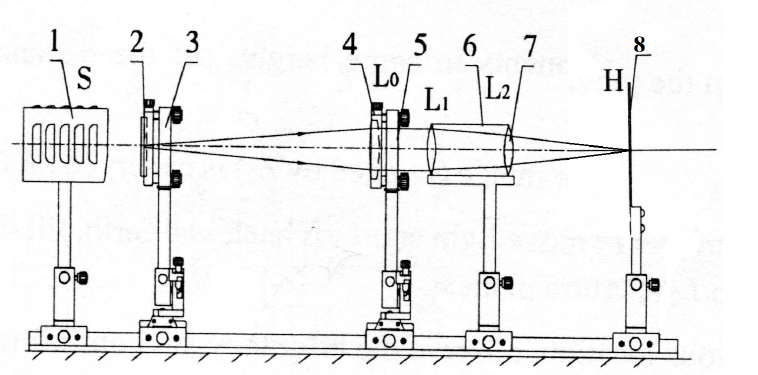
\includegraphics[width=0.7\linewidth]{5}
	\caption{Оптическая система}%Схема расположения оптических элементов в опыте по определению фокусного расстояния оптической системы с помощью метода Аббе. На рисунке изображены следующие элементы: 1~-- осветитель S; 2~-- слайд с линейкой (Millimetre Ruler); 3~-- держатель бипризм (LMP-41); 4~-- линза L0 ($f=150$ мм); 5~-- двухосевой держатель оптических элементов (LMP-07); 6~-- оптическая система, состоящая из линз L1 ($f=190$ мм) и L2 ($f=300$~мм); 7~-- держатель группы линз (LMP-28); 8~-- экран Н (LMP-13)}
	\label{fig:3_1}
\end{figure}
\end{frame}

\begin{frame}
\frametitle{Данные (оптическая система)} 

%План работы: собрали установку (Рис. \ref{fig:3_1}), установили линзу $L_0$ на фокусном расстроении от объекта, получили изображение на бесконечности. За $L_0$ расположили систему линз $L_1-L_2$, расстояние между которыми  $l_{12}$. Двигали экран вдоль оптической оси и находили четкое изображение (экран в этом случае находится в задней фокальной плоскости системы линз). Повернули обе линзы и повторили действие.

%Полученный результат:

\begin{center}
	\begin{tabular}{|c|c|}
		\hline
		№ опыта & Фокусное расстояние F, мм\\
		\hline
		1 & 121 $\pm 0.5$  \\
		\hline
		2 & 118 $ \pm 0.5$ \\
		\hline
	\end{tabular}
\end{center}

После усреднения получим:
$F = 119.5\pm 1.5$ мм

%Теперь определим фокусное расстояние с помощью метода Аббе. Схема опыта представлена на рисунке \ref{fig:3_1}. После эксперимента были получены следующие данные:

\begin{center}
	\begin{tabular}{|c|c|c|}
		\hline
		$\beta_1$ & $\Delta x$, мм & $\beta_2$ \\
		\hline
		1.2 & 20 & 1.5 \\
		\hline
	\end{tabular}
\end{center}

%Тогда по формуле (\ref{eq:1}) получаем:

\begin{equation*}
	F_{abbe} = 120 \text{ мм}
\end{equation*}

%Поскольку фокусные расстояния каждой из линз известны (написаны на их ободе) и равны $F_1 = 190 \text{ мм}$ и $F_2 = 300 \text{ мм}$, по формуле же (\ref{eq:2}), которая выведена для конкретной системы, получим:

\begin{equation*}
	F_{theor} = 126 \text{ мм}
\end{equation*}
\end{frame}

\begin{frame}
\section{Определение углового увеличения телескопа}
\frametitle{Определение углового увеличения телескопа} 

%В настоящей работе изучается модель астрономической зрительной
%трубы. Этот оптический прибор состоит из двух основных частей: объектива
%— линзы, обращённой к объекту, и окуляра — линзы, обращённой к
%наблюдателю. Объектив, в качестве которого используется положительная
%линза, создаёт действительное изображение предмета. Это изображение
%рассматривается глазом через окуляр. Ход лучей в астрономической
%зрительной трубе (трубе Кеплера) представлен на Рис. \ref{fig:4_1}.

\begin{figure}[H]
	\centering
	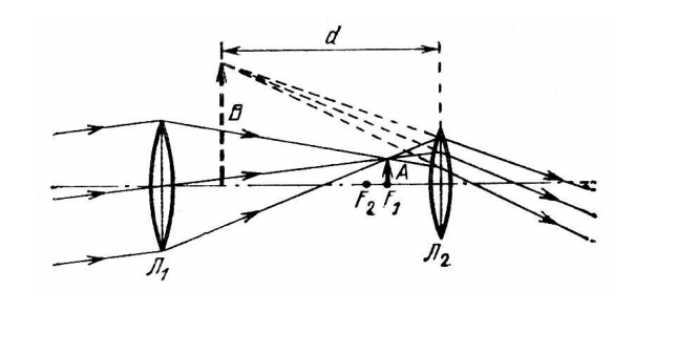
\includegraphics[width=0.6\linewidth]{7}
	\caption{Ход лучей в трубе Кеплера}
	\label{fig:4_1}
\end{figure}

%Для определения углового увеличения телескопа было сделано следующее.

%После слайда-линейки, который выступает в роли объекта, была установлена на ее фокусном расстоянии линза. Это позволяет получить параллельный пучок света, с которым обычно и работают при использовании телескопа. После этого с помощью зрительной трубы было определено число штрихов на линейке $N_1 = 8$, которые укладывались в поле зрения трубы. Затем после линзы была установлена собранная труба Кеплера ($F_1 = 190 \text{ мм, } F_2 = 105 \text{ мм}$) и данная операция была проделана еще раз, с получившимся $N_2 = 4$.

%Угловым увеличением в таком случае по определению будет являться:

\begin{equation}
	\gamma_N = \frac{N_1}{N_2} = 2
\end{equation}
 %С другой стороны, угловое увеличение телекопа равно  отношению фокусов объектива и окуляра:

\begin{equation*}
	\gamma_f = \frac{F_1}{F_2} = 1.81
\end{equation*}
\end{frame}



\end{document}